
\documentclass{frontiersSCNS} % for Science articles

\usepackage{url}
\usepackage[modulo]{lineno}
\linenumbers

%----------------------------------------------------------------------
% Own stuff
\newcommand{\INLINEFIGS}{} % comment out for Frontiers submission
%\usepackage{endfloat}
\usepackage{ucs}
\usepackage[utf8x]{inputenc}
\usepackage{xspace}
\usepackage{textcomp}
\newcommand{\permil}{\,\textperthousand\xspace}
\newcommand{\tbw}[1]{{\bf\parindent0pt\color{red}#1}}
\usepackage{minted}
\newminted{python}{showspaces=false,
  showtabs=false,
%  linenos=true,
  fontsize=\tiny,
  mathescape=true,
  frame=leftline,
  framerule=0pt,
  framesep=0mm}
\ifdefined\INLINEFIGS
\newcommand{\Figure}[2]{Figure~\ref{#2}}
\else
\newcommand{\Figure}[2]{Figure~#1}
\fi
%----------------------------------------------------------------------

\copyrightyear{}
\pubyear{}

\def\journal{Neuroinformatics}%%% write here for which journal %%%
\def\DOI{}
\def\articleType{Research Article}
\def\keyFont{\fontsize{8}{11}\helveticabold }
\def\firstAuthorLast{Djurfeldt {et~al.}}
\def\Authors{Mikael Djurfeldt\,$^{1,2,*}$, Andrew P. Davison\,$^{3}$,
 and Jochen M. Eppler\,$^4$}
% Affiliations should be keyed to the author's name with superscript
% numbers and be listed as follows: Laboratory, Institute, Department,
% Organization, City, State abbreviation (USA, Canada, Australia), and
% Country (without detailed address information such as city zip codes
% or street names).  If one of the authors has a change of address,
% list the new address below the correspondence details using a
% superscript symbol and use the same symbol to indicate the author in
% the author list.
\def\Address{$^{1}$PDC Center for High-Performance Computing, KTH
  Royal Institute of Technology, Stockholm, Sweden\\
  $^{2}$International Neuroinformatics Coordinating Facility (INCF),
  Stockholm, Sweden\\
  $^{3}$Unité de Neurosciences, Information et Complexité (UNIC),
  CNRS, Gif sur Yvette, France\\
  $^{4}$Institute of Neuroscience and Medicine (INM-6) and Institute
  for Advanced Simulation (IAS-6), Jülich Research Centre and
  JARA, Jülich, Germany}
% The Corresponding Author should be marked with an asterisk Provide
% the exact contact address (this time including street name and city
% zip code) and email of the corresponding author
\def\corrAuthor{Mikael Djurfeldt} \def\corrAddress{International
  Neuroinformatics Coordinating Facility (INCF), Nobels väg 15 A,
  Stockholm, SE-17177, Sweden} \def\corrEmail{djurfeldt@incf.org}

% \color{FrontiersColor} Is the color used in the Journal name, in the
% title, and the names of the sections

\begin{document}
\onecolumn
\firstpage{1}

\title[The connection generator API]{Efficient generation of connectivity in
  neuronal networks from simulator-independent descriptions}
\author[\firstAuthorLast ]{\Authors}
\address{}
\correspondance{}
\extraAuth{}% If there are more than 1 additional author, comment this
%line and uncomment the next one
%\extraAuth{corresponding Author2 \\ Laboratory X2, Institute X2,
%Department X2, Organization X2, Street X2, City X2 , State XX2 (only
%USA, Canada and Australia), Zip Code2, X2 Country X2,
%email2@uni2.edu}
\topic{Python in Neuroscience II}

\maketitle
\begin{abstract} % maximum 2000 characters including spaces

Simulator-independent descriptions of connectivity in neuronal
networks promise greater ease of model sharing, improved
reproducibility of simulation results, and reduced programming effort
for computational neuroscientists.  However, until now, enabling the
use of such descriptions in a given simulator in a computationally
efficient way has entailed considerable work for simulator developers,
which must be repeated for each new connectivity-generating library
that is developed.

We have developed a generic connection generator interface that
provides a standard way to connect a connectivity-generating library
to a simulator, such that one library can easily be replaced by
another, according to the modeller's needs.  We have used the
connection generator interface to connect C++ and Python
implementations of the Connection-set Algebra to the NEST simulator.
We also demonstrate how the simulator-independent modelling framework
PyNN can transparently take advantage of this, passing a connection
description through to the simulator layer for rapid processing in C++
where a simulator supports the connection generator interface and
falling-back to slower iteration in Python otherwise.  A set of
benchmarks demonstrates the good performance of the interface.

\tiny
 \keyFont{ \section{Keywords:} model description, connectivity,
 neural simulation, CSA, NEST, PyNN, Python, large-scale modeling}
\end{abstract}

\section{Introduction}

The central nervous systems of vertebrates and many invertebrates have
complex patterns of connections.  In developing neuronal network
models of such systems, there are two main tasks related to connection
patterns. The first is to express the connectivity in a
machine-readable format, e.g. in code or in a configuration file.  The
second is to explain the connectivity unambiguously in prose in an
article or book, so that the model can be understood and reproduced by
someone else \citep{nordlie-2009_e1000456}.

For expressing connectivity in code, three methods are commonly used:
(i) procedural code written by the modeller, using low-level
operations such as connecting pairs of neurons or connecting a single
neuron to a group; (ii) a library of pre-defined, parameterized
connection routines; (iii) an explicit list of connections.  Each of
these have their limitations.  Procedural code and libraries limit the
connectivity descriptions to a single language and often a single
simulator, making it hard to port models from one simulator to
another.  Procedural code takes time to write, and will have more bugs
than a library, since library code is likely to be more thoroughly
tested and reused.  On the other hand, the connectivity patterns
available from a library are inevitably more limited than those that
can be achieved with user-written code.  Using an explicit list of
connections is largely independent of a particular simulator or
programming language, but may cause problems of storage and
input/output efficiency, and does not enable conceptual descriptions
of connectivity.  All of these methods make it difficult to explain
the connectivity in a scientific text. For a fuller discussion of
these issues see \citet{crook12}.

These problems can be reduced or avoided by using a general purpose
connectivity-generating software library such as the Connection-set
Algebra \citep[CSA;][]{djurfeldt12} or the NineML graph library
\citep{raikov10}.  Such libraries allow simulator-independent
specification of connectivity and enable high-level, declarative
descriptions which do not constrain how the connectivity should be
realized in code and hence give scope for optimization and
parallelization within the simulator software.  The CSA in addition
supports succinct, unambiguous descriptions of connectivity in text,
using a mathematical notation.

The adoption of new, simulator-independent methods for expressing
connectivity, such as CSA, is hindered by the effort needed to add
support for a given connectivity-generating library to a simulator.
This effort must, in general, be repeated for each simulator that
wishes to support the library.  The exception to this is if using a
simulator-independent modelling interface such as PyNN
\citep[\url{http://www.neuralensemble.org/PyNN};][]{Davison09}, which
supports multiple simulators; PyNN however is written in Python, which
means that processing the CSA description will be slower than if using
C/C++ (the languages in which many simulators are written).
Furthermore, whether using a simulator-independent interface or not, a
new programming effort is needed if another new method for expressing
connectivity is developed.

To minimize the effort required of simulator software developers, and
allow modellers to flexibly choose among simulators and libraries
which generate connectivity, we have developed a generic
\emph{connection generator} interface, which enables the use of CSA
and similar libraries in different neuronal simulators.  The interface
makes both the simulator and the connectivity-generating library
replaceable and therefore gives maximum flexibility to the modeller.

In this article we first describe the connection generator interface.
As an example of a connectivity-generating library, we then give a
brief overview of CSA and of different software libraries that support
using CSA in Python and C++ code. We show how the connection generator
interface has been integrated in the NEST simulator
\citep[\url{http://www.nest-simulator.org};][]{Gewaltig_07_11204},
enabling the use of connection libraries such as CSA, before
describing its use from higher software layers, such as the PyNN
framework.  Finally, we provide benchmarks for different use case
scenarios of the interface.

%----------------------------------------------------------------------

\section{The connection generator interface}\label{sec:conn_gen}

To allow users to flexibly choose among simulators and libraries which
generate connectivity, we have developed an interface that abstracts the
simulator and the connectivity-generating library from each other,
making both the simulator and the connectivity description library
replaceable.

\ifdefined\INLINEFIGS
\begin{figure}[ht]
\centering
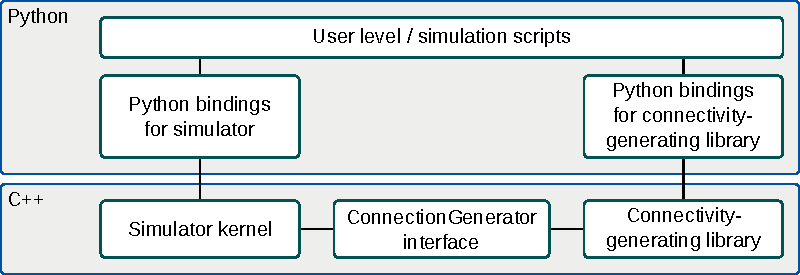
\includegraphics[scale=.8]{figures/block_diagram_conngen.pdf}
\caption{Block diagram of the connection generator interface and the
  components involved. The central component is the
  \texttt{ConnectionGenerator} class itself. It can connect to different
  simulators (e.g. NEST) and to different connectivity-generating
  libraries (e.g. CSA). In this example, Python is used as scripting
  language for both simulator and connectivity-generating
  library.}\label{fig:block_diagram_conngen}
\end{figure}
\fi

A connectivity-generating library, such as \verb|csa| or \verb|libcsa|
of Section~\ref{sec:impl}, is used to create an object representing
network connectivity.  In the case of a CSA library, this object is a
connection-set, but it could also be a graph constructed from graph
primitives. The connection generator interface provides a C++ level
interface to such objects which allows software external to the
connectivity-generating library to efficiently iterate through
connections represented by the object.  In the example shown in
\Figure{2}{fig:block_diagram_conngen}, the connection generator
interface is used to combine a Python-scripted simulator with a
Python-scripted connectivity-generating library.  A connectivity
generating object is assembled at the Python level.  If \verb|libcsa|
is used, the resulting object will be a C++ object with a Python
wrapper (see lower two boxes to the right in the figure). The object
is used by a C++ simulator kernel (lower box to the left) to specify
network connectivity. By providing connectivity-generating software
that implements the connection generator interface as dynamically
linked libraries, multiple such libraries can be loaded into the
Python runtime environment and even used simultaneously without a need
to recompile the simulator.

\subsection{The interface}\label{sec:cgint}

In neuronal network simulations we often want to specify a
``projection'' between a source population of neurons and a target
population.  A projection consists of many individual connections
between the populations.  In nature, one such connection corresponds
to an axon forming a synaptic contact on the spine/dendrite of a
receiving neuron.  A \verb|ConnectionGenerator| object is modeled on
the concept of a projection.  The source and target populations are
each enumerated using consecutive, non-negative integer indices
starting from 0.  These indices are used to specify source and target
neuron identity for a connection and constitute an abstraction barrier
between the actual elements of a population and the connection
generator.  This allows the elements to be either neurons (appropriate
for networks of point neurons) or individual synapses (appropriate for
networks with morphologically-detailed neurons).

The principle of operation of the connection generator interface is an
iteration over connections represented by the object.  A simulator, or
other software using a connection generator, repeatedly calls a
function \verb|next()| until boolean \verb|false| is
returned. Connections are represented by source and target index,
together with zero or more connection parameters.  The number of
parameters is called the \emph{arity} of the
\verb|ConnectionGenerator|.

Connection generators can be flexible with regard to the sizes of the
source and target populations. The source and target index sets that
should be iterated over for the populations at hand are each specified
through the interface as a \emph{mask}.  In the case of a parallel
simulator, a specific mask is given per MPI rank.  Typically, the
source index set is the same in all such masks while the target index
sets are unique for each rank and non-overlapping.  Each rank should
provide all masks (i.e. the set of masks for all ranks). Some
connection generators can use such information to avoid the need for
communication with other ranks.

The interface is designed as an abstract base class in C++
and consists of the following virtual functions:

\begin{unlist}
\item[\tt int arity()]: return the number of per-connection values
  associated with this generator. Values can be parameters like
  weight, delay, time constants, or others.
\item[\tt int size()]: return the number of connections represented by
  this generator.
\item[\tt void setMask(Mask\& mask)]: inform the generator about which
  source and target indices are available. A
  \verb|ConnectionGenerator| mask represents the available nodes in
  the network for which to create connections.
\item[\tt void setMask(std::vector$<$Mask$>$\& masks, int local)]:
  this version of \texttt{setMask} is used by parallel simulators and
  informs the connection generator on the \verb|local| rank about the
  masks of all ranks. Different ranks usually have different masks
  since they are responsible for different subsets of the connections
  of the network. Some connection generators can use such information
  to avoid the need for communication with other ranks.
\item[\tt void start()]: start an iteration. This function must be called
  before the first call to \verb|next()|.
\item[\tt bool next(int\& source, int\& target, double* value)]:
  advance to the next connection or return false, if no more
  connections are available from the \verb|ConnectionGenerator|.
  Source and target indices of the connection as well as associated
  parameters are written into \verb|source|, \verb|target| and the
  array pointed to by \verb|value|, respectively. The order of
  iteration is according to increasing index, with all sources
  iterated over per target.
\end{unlist}

\subsection{libneurosim}\label{sec:libneurosim}
If the C++ header file for the connection generator interface
definition and its supporting code were placed in the simulator or
connectivity-generating library source trees, it would be duplicated
over simulators or libraries.  As new versions of the interface are
developed, the situation would quickly become unmanageable. The
connection generator interface is unusual in that it is a symmetric
abstraction barrier: it both allows a given simulator to use any
library supporting the API \emph{and} allows the same library to be
used from any simulator supporting the API.

To create a space in which to put interfaces and other code of generic
use for neuronal network simulation software, we have developed the
neurosim library
(\url{http://software.incf.org/software/libneurosim}).  More
precisely, libneurosim is a software package which currently consists
of two main component libraries: \verb|libneurosim|, providing C++
level support code and \verb|libpyneurosim|, providing Python support
code.

\verb|Libneurosim| provides the \verb|ConnectionGenerator| interface
(\Figure{2}{fig:block_diagram_conngen}, bottom). It also contains a
registry for XML parser functions.  Different types of connection
generators can be described by different XML-based languages.  For
example, the \verb|csa| library can serialize connection-set
expressions using a MathML-based language.  A connectivity-generating
library may provide a parser for one or more such languages.
Conversely, the same XML-based language might be used by one or more
connectivity-generating libraries.  The XML parser registry maps XML
tags identifying specific languages to specific connection libraries.
The interface to the registry consists of three static methods in the
connection generator interface:

\begin{unlist}
\item[\tt void selectCGImplementation (std::string tag, std::string
  library)]:\\ Associate the parent node tag \verb|tag| with the library
  \verb|library|.  The library named \verb|library| will be
  dynamically loaded and will invoke the \verb|libneurosim| function
  \verb|registerConnectionGeneratorLibrary| to register its XML
  parser.
\item[\tt ConnectionGenerator* fromXML (std::string xml)]: Parse the
  XML representation \verb|xml| of a connection generator and return
  it. The function dispatches to parsers of different libraries
  depending on previous calls to \verb|selectCGImplementation|.
\item[\tt ConnectionGenerator* fromXMLFile (std::string fname)]: Same
  as previous function, but read the XML stream from the file with
  pathname \verb|fname|.
\end{unlist}

\verb|libpyneurosim| currently contains generic support for
registering new Python connection generator types and unwrapping
instances of such objects:

\begin{unlist}
\item[\tt void registerConnectionGeneratorType (CheckFuncT,
  UnpackFuncT)]: Register a new type checking and unwrapping
  function.
\item[\tt isConnectionGenerator (PyObject* pObj)]: Check if
  \verb|pObj| is a known connection generator type (as identified by
  previously registered checking functions).
\item[\tt ConnectionGenerator* unpackConnectionGenerator (PyObject*
  pObj)]: Unwrap the connection generator in \verb|pObj| and return
  it.
\end{unlist}

\section{The connection-set algebra}\label{sec:csa}

The connection generator interface described in the previous section
enables the simulators to use external connectivity-generating
libraries. The benchmarks in Section~\ref{sec:benchmarks} use the
interface to couple NEST to the connectivity-generating libraries
\verb|csa| and \verb|libcsa|, which we now introduce.

The Connection-set Algebra is a declarative formalism for the
specification of network connectivity which can be used both when
describing a network to a fellow researcher and when implementing a
model for a simulator. CSA expressions define connection-sets. A
connection-set is the set of edges in a network graph, together with
parameters associated with those edges. The abstract nature of CSA
creates a clean separation between CSA and other aspects of model or
simulator infrastructure.  CSA expressions consist of pre-defined
elementary connection-sets and operators such that new connection-sets
can be defined in terms of existing ones. It enables a succinct and
precise description and definition of connectivity in terms of such
expressions. By allowing connection-sets to be infinite, they can
represent \emph{types} of connectivity---connectivity patterns---in
addition to connectivity of specific networks. There are ways to
implement CSA on a computer which are both efficient and scalable on a
parallel computer, also when connection-sets have infinite size. The
parallelization is transparent to the user since intersection
operators in the algebra can efficiently subdivide a connection-set
among processes.

CSA is currently focused on connectivity which has a constructive or
statistical element such as connectivity specified by an algorithm,
but it can also be used when all network connections are given
explicitly or in cases where only some elements of the connectivity
are explicitly specified.

\subsection{Connection-sets}

To give a flavor of CSA, we will now further introduce some of its
concepts.  Given source and target populations $P_s$ and $P_t$, a CSA
connection-set is defined as the set of connections between $P_s$ and
$P_t$ along with zero or more per-connection parameters such as weight
or delay. As for connection generators, elements of populations are
enumerated using non-negative integers. Thus, a population $P$ is
represented by an index set $\mathcal{I}$. One connection from $P_s$
to $P_t$ is represented by the pair $(i, j)$, where $i \in
\mathcal{I}_s, j \in \mathcal{I}_t$.  Such indices are similar to the
GIDs (Global IDentifiers) of the NEURON and NEST simulators but
normally start at 0 and run consecutively for each population.
Introducing this abstraction, in the form of a mapping from objects in
the simulation domain to integers, gives at least two major
advantages: 1. The CSA does not need to care about the nature of the
objects in $P$---they could just as well be synaptic boutons as
neurons.  2. The index set $\mathcal{I}$ can be chosen to be
infinite. This is useful when generically specifying a connectivity
pattern independent of the sizes of the specific source and target
populations for which it will later be used. This is further discussed
in Section~\ref{sec:structure}.

\ifdefined\INLINEFIGS
\begin{figure}[ht]
\centering
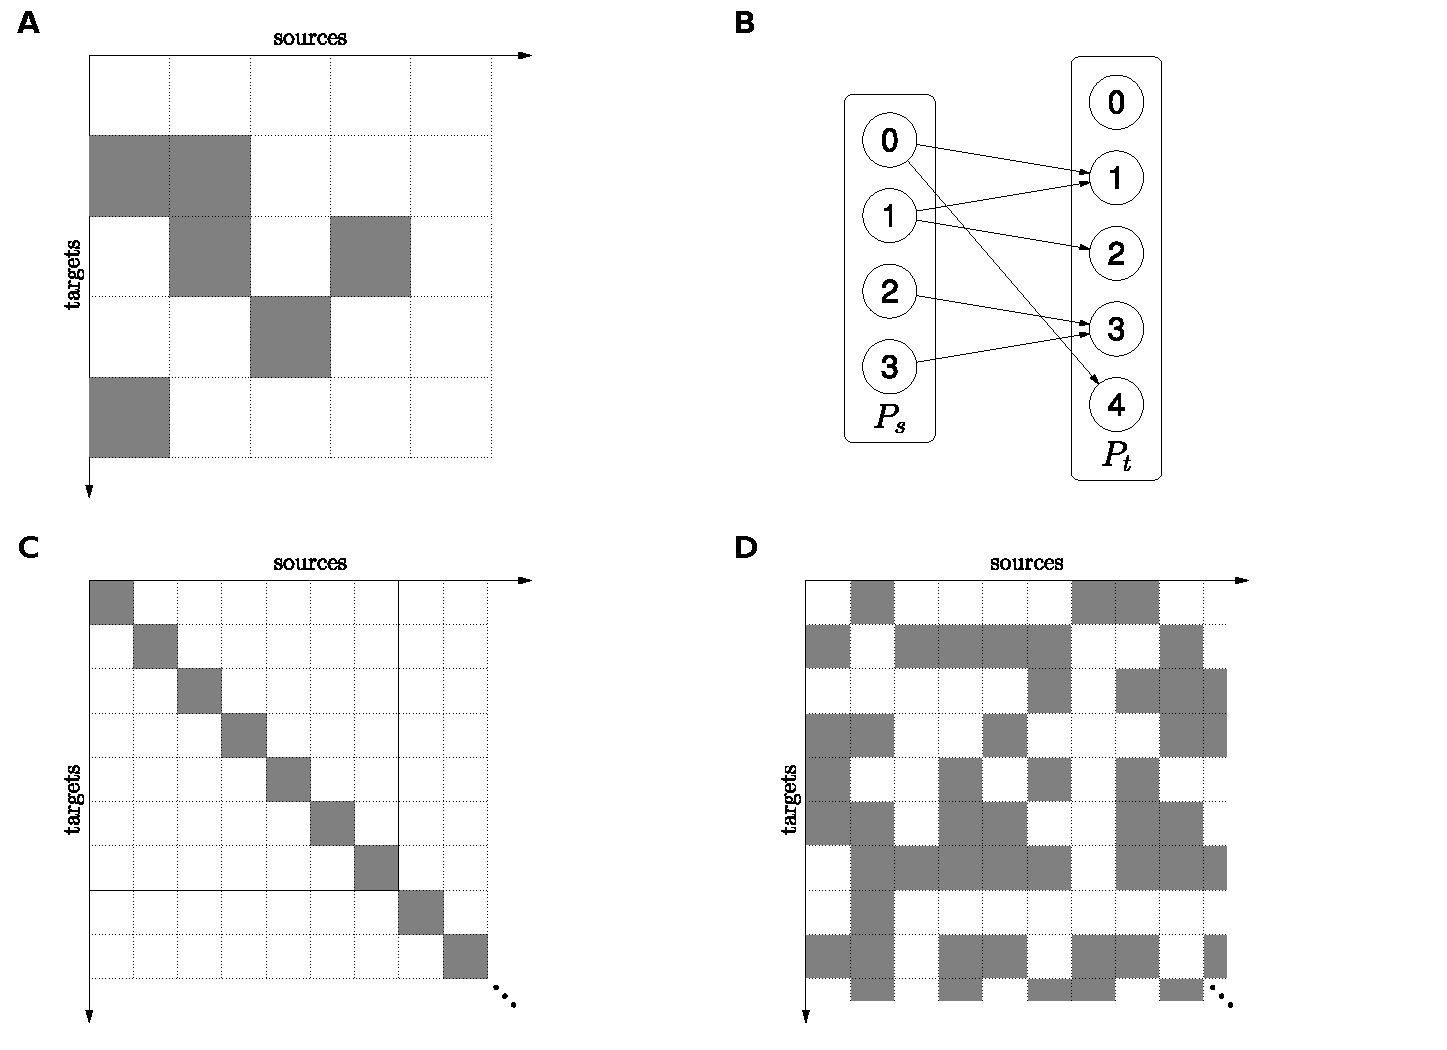
\includegraphics[scale=.7]{figures/csa-pane.pdf}
\caption{
  \textbf{A} The mask $\overline{M} =
  \{(0,1), (1,1), (1,2), (3,2), (2,3), (0,4)\}$ shown as a connection
  matrix. Grey squares represent existing connections.
  \textbf{B} Network connectivity when the mask in A is applied to
  source population $P_s$ and target population
  $P_t$.
  \textbf{C} The one-to-one mask $\bar{\delta}$. The mask is infinite,
  but finite portions can be cut out when applied to finite source and
  target populations. This is illustrated by the solid square for
  source and target size 7. When source and target population is the
  same, $\bar{\delta}$ represents self-connections.
  \textbf{D} The mask $\bar{\rho}(0.5) - \bar{\delta} =$ random
  connectivity without self-connections.
}\label{fig:csa} 
\end{figure}
\fi

A connection-set with zero parameters is called a \emph{mask}. A mask
states which connections exist.  In the example of the mask
$\overline{M} = \{(0,1), (1,1), (1,2), (3,2), (2,3), (0,4)\}$ it can
be regarded either as a connection matrix (see \Figure{1}{fig:csa}A)
or as a boolean indicator function:
\begin{equation*}
\overline{M} : \mathcal{I}_s \times \mathcal{I}_t \rightarrow \{ \mathcal{F},
\mathcal{T} \}
\end{equation*}
In the example $\overline{M}(0,0) = \mathcal{F}$ while
$\overline{M}(1,1) = \mathcal{T}$. If the mask is combined with a
source population $P_s$ and a target population $P_t$, the result is
the network $(P_s, P_t, \overline{M})$ shown in \Figure{1}{fig:csa}B.

In CSA, connections can be parameterized through functions mapping
connections to values:
\begin{equation*}
V : \mathcal{I}_s \times \mathcal{I}_t \rightarrow \mathcal{V}
\end{equation*}
where $\mathcal{V}$ is some codomain. In \citet{djurfeldt12}, such a
function is called a \emph{value set}. An example of a value set is
distance dependent delays with added noise sampled from a clipped
random normal distribution. Value sets are typically used to assign a
weight or delay to connections.

A CSA \emph{connection-set}, $C$, is a tuple of a mask and zero or
more value sets:
\begin{equation*}
C = (\overline{M}, V_0, V_1, ...)
\end{equation*}
The number of value sets of a connection-set is called its
\emph{arity}. A connection-set with arity 0 is for all purposes
equivalent to a mask and the two can be used interchangeably.

\subsection{An algebra for connectivity structure}\label{sec:structure}

In CSA, the concepts defined in the previous section have been
developed into a formalism for describing connectivity structure.
Assume that a mask specifies connectivity for a single population such
that $P_s = P_t = P$ and that we are interested in describing
self-connections, i.e. every neuron in $P$ should be connected to
itself.  If the size of $P$ is 4, the mask $\{(0, 0), (1, 1), (2, 2),
(3, 3)\}$ could be used.  If the size is 2, the mask $\{(0, 0), (1,
1)\}$ would be appropriate. Such masks contain not only information
about connectivity structure but also about population size. We can
generalize by stripping off the population size information and
allowing the index set $\mathcal{I}$ and mask to be infinite, defining
the one-to-one mask $\bar{\delta}$:
\begin{equation*}
  \bar{\delta}(i, j) =
      \begin{cases}
        \mathcal{T}& \text{if $i = j$},\\
        \mathcal{F}& \text{otherwise}.
      \end{cases}
      \quad i, j \in \mathcal{I} = \mathbb{N}_0
\end{equation*}
Now $\bar{\delta}$ only encapsulates the concept of self- or
one-to-one connectivity structure (depending on whether the source and
target populations are the same or different) without reference to
size, i.e. we can describe a \emph{type} of connectivity independently
of any specific network.  Finite portions can be cut out of such
infinite connection-sets when applied to finite populations (see
\Figure{1}{fig:csa}C).

CSA provides a set of elementary connection-sets such as
$\bar{\delta}$. Another example is the random mask $\bar{\rho}$, a
parameterized connection-set, or, more strictly, a mask-valued
function $\bar{\rho}(p)$ where the parameter $p$ is the probability
that a given connection $(i, j)$ exists.  That is, for each
combination of pre- and post-synaptic neurons, a Bernoulli trial
determines whether they are connected.
\begin{equation*}
  \bar{\rho} (p) (i, j) =
  \begin{cases}
    \mathcal{T}& \text{with probability $p$},\\
    \mathcal{F}& \text{otherwise}.
  \end{cases}
  \quad i, j \in \mathbb{N}_0
\end{equation*}
By using CSA \emph{operators} such as intersection ($\cap$), union
($\cup$) and set difference ($-$), connection-sets can be combined into
expressions. For example, the idea of ``random Erd\H{o}s-R\'enyi
connectivity without self-connections'' can be represented by the CSA
expression $\bar{\rho}(p) - \bar{\delta}$ (see Figure
\ref{fig:csa}D). A mask representing all possible connections between
two finite populations can be formed by taking the Cartesian product
of their index sets, $\mathcal{I}_s \times
\mathcal{I}_t$. Intersecting with this mask can turn an infinite
connection-set, representing connectivity structure, into a connection
matrix between the populations. For example, the finite part of the
matrix in \Figure{1}{fig:csa}C is $\{0..6\} \times \{0..6\} \cap
\bar{\delta}$. For a more in-depth description of the CSA and
principles of implementation see \citet{djurfeldt12}.

%  \textbf{Figure 1.}{CSA Connection Matrix.}\label{fig:01}
%\subsection{Examples}
%  \textbf{Figure 2.}{An example of using CSA.}\label{fig:02}
%\subsection{Parallelization}
\subsection{Implementations}\label{sec:impl}

There currently exist three implementations of CSA.  They internally
represent connection-sets as iterators and CSA expressions as trees of
such iterators, although


The original
implementation is written in C++ and is part of the SPLIT simulation
library \citep{djurfeldt05}.  It was used to specify the connectivity
of the KTH cortex model \citep{djurfeldt08}---a model with three
hierarchical levels of structure.  The second implementation is
written in Python and is available as the Python library \verb|csa|.
Here, the aims were 1. to get an easily usable and extensible
demonstration of CSA and 2. to experiment with new ways to implement
CSA. This implementation has been released as free software under the
GPL and is available at the INCF software center
(\url{http://software.incf.org/software/csa}). A third implementation
in C++, \verb|libcsa|, is currently under development and will also be
released under the GPL. It provides Python bindings such that CSA
objects can be formed by Python level expressions with similar syntax
as used with the \verb|csa| library. For further information about
this syntax, the reader is referred to the tutorial in the \verb|csa|
package. The benchmarks in this article (Section~\ref{sec:benchmarks})
were performed using the latter two implementations in Python and C++,
\verb|csa| and \verb|libcsa|.

% MDJ: I think I'll keep it like that. This paper is so complex
% conceptually anyway. We don't need to desribe everything!

%\subsubsection{Masks}
%\subsection{Python wrapper}
%\subsection{Serialization/deserialization}

%----------------------------------------------------------------------

\section{Using connection generators in NEST}\label{sec:conn_gen_nest}

NEST is a simulator for large networks of point neurons or neuron
models with few electrical compartments
\citep[\url{http://www.nest-simulator.org};][]{Gewaltig_07_11204}. It
is suited for a broad range of neuronal network modeling approaches
and runs on a large variety of computer architectures. NEST is
parallelized using OpenMP \citep{OpenMPSpec} and MPI
\citep{MPIForum94} and scales well on ordinary desktop computers to
large clusters of multi-core processors and supercomputers
\citep{Helias12_26}.

The network description is a script, written either in SLI, NEST's
built-in simulation language, or in Python, using the Python interface
to NEST \citep[PyNEST;][]{Eppler09_12}. To build a network in NEST,
the user first creates the neurons of the network and devices for
stimulation and measurement using the \verb|Create| function and then
connects the elements with each other.

\subsection{Native connection functions}

The most basic way to set up connections is using the \verb|Connect|
function, which takes a list of pre-synaptic neurons (or devices) and
a list of the same amount of post-synaptic neurons (or devices) and
connects the corresponding elements in a one-to-one fashion. Because
of the function call overhead, this function is not very efficient to
use when creating large networks.

To avoid such overhead, the functions \verb|ConvergentConnect| and
\verb|DivergentConnect| can be used to create multiple connections
with a single call. In addition, random variants for both of these
functions exist to support the user in creating networks on the basis
of knowledge of connectivity statistics. However, random connection
parameters (e.g. \emph{weight}, \emph{delay}, or time constants) need
to be specified by user code and supplied to NEST after the creation
of connections.

\subsection{Topology module}

To ease the creation of networks with topological relations between
the neurons and organizations of neurons into layers and areas, NEST
provides a Topology module \citep{Plesser_13}. It supports the user in
connecting neurons and randomly initializing synapse parameters based
on geometry or topological relationships in the network. A comparison
between the native connection routines, the Topology module of NEST,
and the novel connection generator interface described below is
subject to future work.

\subsection{Connectivity-generating libraries}

As detailed above, NEST provides multiple methods for connecting
neurons into a network. However, while the native routines scale very
well \citep{Helias12_26}, they are only suitable for creating simple
patterns such as convergent/divergent connectivity without looping
over them in user code. On the other hand, the topology module
\citep{Plesser_13} allows the creation of more complex structures, but
requires neurons to be organized in special data structures (e.g.
layers). This has some overhead, which is reflected in the
performance and scaling.

To support the connection generator interface in NEST and thus make
more connectivity-generating libraries available to users, we created
the \verb|ConnectionGeneratorModule|. It is implemented as a plugin
for NEST which extends both user interfaces, SLI and PyNEST, and
builds on \verb|libneurosim| (see Section~\ref{sec:libneurosim}).

All neurons and devices in NEST are identified uniquely by an integer
number, their global id (\emph{GID}). As all existing connection
routines in NEST work either on single GIDs or on lists of GIDs, we
decided to also use this convention for the connection generator
interface in NEST, although that itself uses indices starting from
zero (see Section~\ref{sec:cgint}). Our new connection generator
interface for NEST consists of the following functions:

\begin{unlist}
\item[{\tt CGConnect} ] takes a \verb|ConnectionGenerator| \emph{cg},
  lists of GIDs for \emph{pre}- and \emph{post}-synaptic
  populations, and a \emph{param\_map}. It creates the connections
  between neurons in \emph{pre} and \emph{post} as prescribed by
  the rules in \emph{cg}. The parameter map \emph{param\_map} maps
  parameter names (e.g. \emph{weight}, \emph{delay}) to their index
  for the parameter value vector created by the call to \verb|next()|
  in the connection generator interface (see Section
  \ref{sec:cgint}).
\item[{\tt CGParse} ] takes a serialized version of a connection
  generator in the string \emph{xml} and returns the corresponding
  \verb|ConnectionGenerator| object. A special use of this function
  exists on supercomputers, where Python is often not available on the
  compute nodes, or where the memory and performance penalty would not
  be acceptable and a pure SLI-based solution is preferable.
\item[{\tt CGParseFile} ] takes a file name \emph{fname} and parses the
  serialized version of a connection generator contained therein.
\item[{\tt CGSelectImplementation} ] takes an XML tag \emph{tag}
  representing the parent node of a serialized connection generator
  and the name of a library \emph{library} to provide a parser for
  such an XML file. This information determines which library should
  carry out the parsing for \verb|CGParse| and \verb|CGParseFile|.
\end{unlist}

In order to use the new interface in NEST, the user first has to
construct a \verb|ConnectionGenerator| object.
This can be done at the Python level by either using
\verb|csa| or the Python bindings of \verb|libcsa| (see
Section~\ref{sec:impl}). When PyNEST is used, this object can directly
be given to \verb|CGConnect|, which wraps the
\verb|ConnectionGenerator| object into a SLI Datum of type
\verb|connectiongeneratortype| that can be shipped into NEST's
simulation kernel. It is then iterated on the C++ level in case of
\verb|libcsa|, or by calling back into Python in case of \verb|csa|.

Another way to construct a \verb|ConnectionGenerator| object is by
parsing an XML serialization of the object. Such a serialization could
be created at the Python level, created by an external tool, or
written by hand.  At the SLI level
this serialization can then be given to one of the
SLI functions \verb|CGParse| or \verb|CGParseFile|, which
reinstantiate the original object using the functions \verb|fromXML| or
\verb|fromXMLFile| in the connection generator API. This object (of type
\verb|connectiongeneratortype|) can be given to SLI's version of the
\verb|CGConnect| function. Please note that the step of creating the
serialization of the \verb|ConnectionGenerator| can also be carried
out on another machine. This allows to run simulations using CSA
on machines where Python is not available.

\ifdefined\INLINEFIGS
\begin{figure}[ht]
\centering
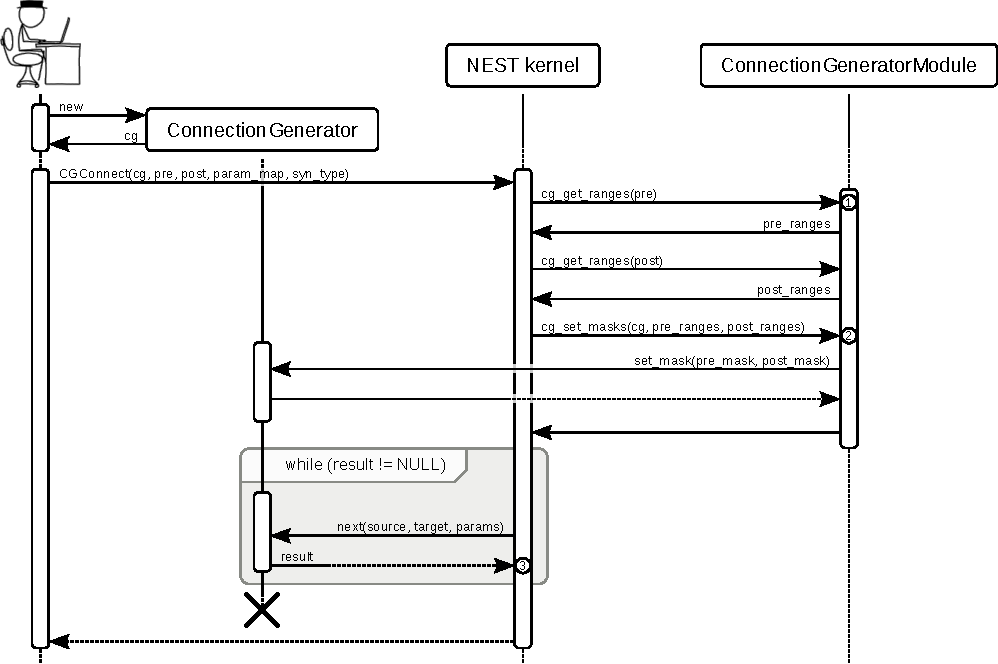
\includegraphics[scale=.8]{figures/sequence_diagram_nest.pdf}
\caption{Sequence diagram showing the function calls during the use of
  the connection generator interface in NEST. The user first creates a
  \texttt{ConnectionGenerator} object \emph{cg}. She then calls
  PyNEST's \texttt{CGConnect()} function. \textcircled{\footnotesize
    1} The function \texttt{cg\_get\_ranges()} returns all contiguous
  ranges of global IDs (GIDs) in the given list as a vector of closed
  intervals, still using the GID representation.
  \textcircled{\footnotesize 2} At this point in time, the
  \texttt{ConnectionGeneratorModule} needs to translate the GIDs to
  CSA indices, which run from 0 and enumerate the elements of the
  given \emph{pre}- and \emph{post}-synaptic populations. The result
  of the translation (\emph{pre\_mask} and \emph{post\_mask}) is used
  to set the masks on \emph{cg}. \textcircled{\footnotesize 3} The
  NEST kernel iterates the connection generator by calling
  \texttt{next()} until there are no more connections. For each
  received connection, it creates the connection by calling
  \texttt{Network::connect()}. If a non-empty \emph{param\_map} was
  given to \texttt{CGConnect}, the connection's weight and delay are
  taken from the value-set in
  \emph{cg}.}\label{fig:sequence_diagram_nest}
\end{figure}
\fi

\Figure{3}{fig:sequence_diagram_nest} shows the different entities in
NEST involved in a user call to \verb|CGConnect| in PyNEST. After
setting the masks for the connection generator to tell it which
neurons are local and which are remote (see Section~\ref{sec:cgint}),
the NEST kernel iteratively calls \verb|next()|. This function returns
source and target indices, and values for weight and delay if the
arity of the connection generator is 2, until there are no more
connections. The connections are internally established one by one by
calling NEST's basic \verb|Network::connect()| function on the C++
level.

%----------------------------------------------------------------------

\section{Using connection generators in PyNN}\label{sec:conn_gen_pynn}

PyNN \citep[\url{http://www.neuralensemble.org/PyNN};][]{Davison09} is
a simulator-independent API for
describing neuronal networks in Python. Given a PyNN/Python model
description, the user can choose which simulator to use without needing
to change the model script. This is achieved through a set of
\emph{simulator backends}.
Each backend is a Python module that implements the API
for a specific simulator, for example by providing a mapping from standard
model names and units in PyNN to simulator-specific ones.

In PyNN, a neuronal network is built from \verb|Population|s of
neurons and \verb|Projection|s between them. Each \verb|Projection| is
created by a \verb|Connector|, which knows how to set up the
individual connections. Different \verb|Connector|s exist and allow to
set up a variety of different deterministic and probabilistic
connection patterns. 

To enable them to be simulator-independent, each \verb|Connector| is
implemented in terms of lower-level commands, typically one-to-one or
convergent connect functions, available in all simulators.  However,
because these commands are low-level this approach entails a certain
performance penalty due to transfer of source/target lists and
connection parameters and function call overhead.

To overcome the problem of excessive data transfers between PyNN and
the simulator, a backend can supply customised \verb|Connector|
implementations that are more efficient than using the default,
simulator-independent implementations.  Such custom implementations
can be iterated and expanded at the simulator level and thus avoid
overhead. Moreover, they allow efficient parallelization at the lower
software layers.  Prior to the creation of the connection generator
interface, however, the limitation of this was that a separate custom
implementation had to be written for each PyNN \verb|Connector|.

Since version 0.7, PyNN has provided the generic \verb|CSAConnector|,
which can iterate a CSA connection set and issue one by one connect
calls to the different simulators through their backends. Internally,
the connector executes the following two steps:

\begin{enumerate}
\item Form a finite connection-set adapted to the actual sizes of the
  populations by intersecting the given connection set with the
  Cartesian product of the neuron indices of the pre- and
  post-synaptic populations.
\item Connect the neurons. The weight, delay and any other synaptic
  parameters are taken from the connection set, if supplied as value
  sets (see Section~\ref{sec:csa}), or from the parameterization of
  the synapse type otherwise.
\end{enumerate}

During this study, we extended the NEST backend for PyNN with a new
and specialized \verb|CSAConnector| which passes the complete
\verb|ConnectionGenerator| object down to the simulator (by calling
PyNEST's \verb|CGConnect| function). The iteration over the
connections can then take place on the C++ level in NEST (see
Section~\ref{sec:conn_gen_nest}). This greatly reduces the overhead
and thus improves the runtime and scalability of connection generation
(see Section~\ref{sec:benchmarks}).

%----------------------------------------------------------------------

\section{Benchmarks}\label{sec:benchmarks}

We ran a series of benchmarks in order to assess the performance of
and compare two implementations of CSA (see Section~\ref{sec:impl})
and the two implementations of the \verb|CSAConnector| for PyNN (see
Section \ref{sec:conn_gen_pynn}). Grouped by the software layer in
which the iteration of the connection generator happens (either in
Python by PyNN or in C++ by NEST, see Section~\ref{sec:conn_gen_nest})
and the CSA implementation used (\verb|csa| is the Python version,
\verb|libcsa| the C++ version), the following scenarios were measured:

\begin{itemize}
\item \textbf{Python, csa} used PyNN's original \verb|CSAConnector|
  that is available for all backends in combination with the Python
  CSA implementation. The \verb|CSAConnector| intersects the
  \verb|csa| object with a mask representing the actual source and
  target nodes available and iterates the \verb|csa| object entirely
  at the Python level. It connects the neurons by issuing
  \verb|ConvergentConnect()| calls to PyNEST.
\item \textbf{C++, csa} used the new \verb|CSAConnector| for PyNN's
  NEST backend, which is available in the development version of PyNN,
  and the Python CSA implementation. The \verb|csa| object is passed
  down to NEST through \verb|CGConnect()|. The
  ConnectionGeneratorModule then iterates it at the C++ level by
  repeatedly calling the Python level iterator.
\item \textbf{Python, libcsa} used the generic \verb|CSAConnector| in
  PyNN and the C++ CSA implementation \verb|libcsa|. The
  \verb|CSAConnector| iterates the \verb|libcsa| object at the Python
  level, repeatedly calling its C++ connection generator.
\item \textbf{C++, libcsa} used the new \verb|CSAConnector| for PyNN's
  NEST backend and the C++ CSA implementation \verb|libcsa|. The
  \verb|libcsa| object is passed down to NEST through
  \verb|CGConnect()|. All iteration happen in C++ in the
  \verb|ConnectionGeneratorModule|.
\end{itemize}

\ifdefined\INLINEFIGS
\begin{figure}[ht]
\centering
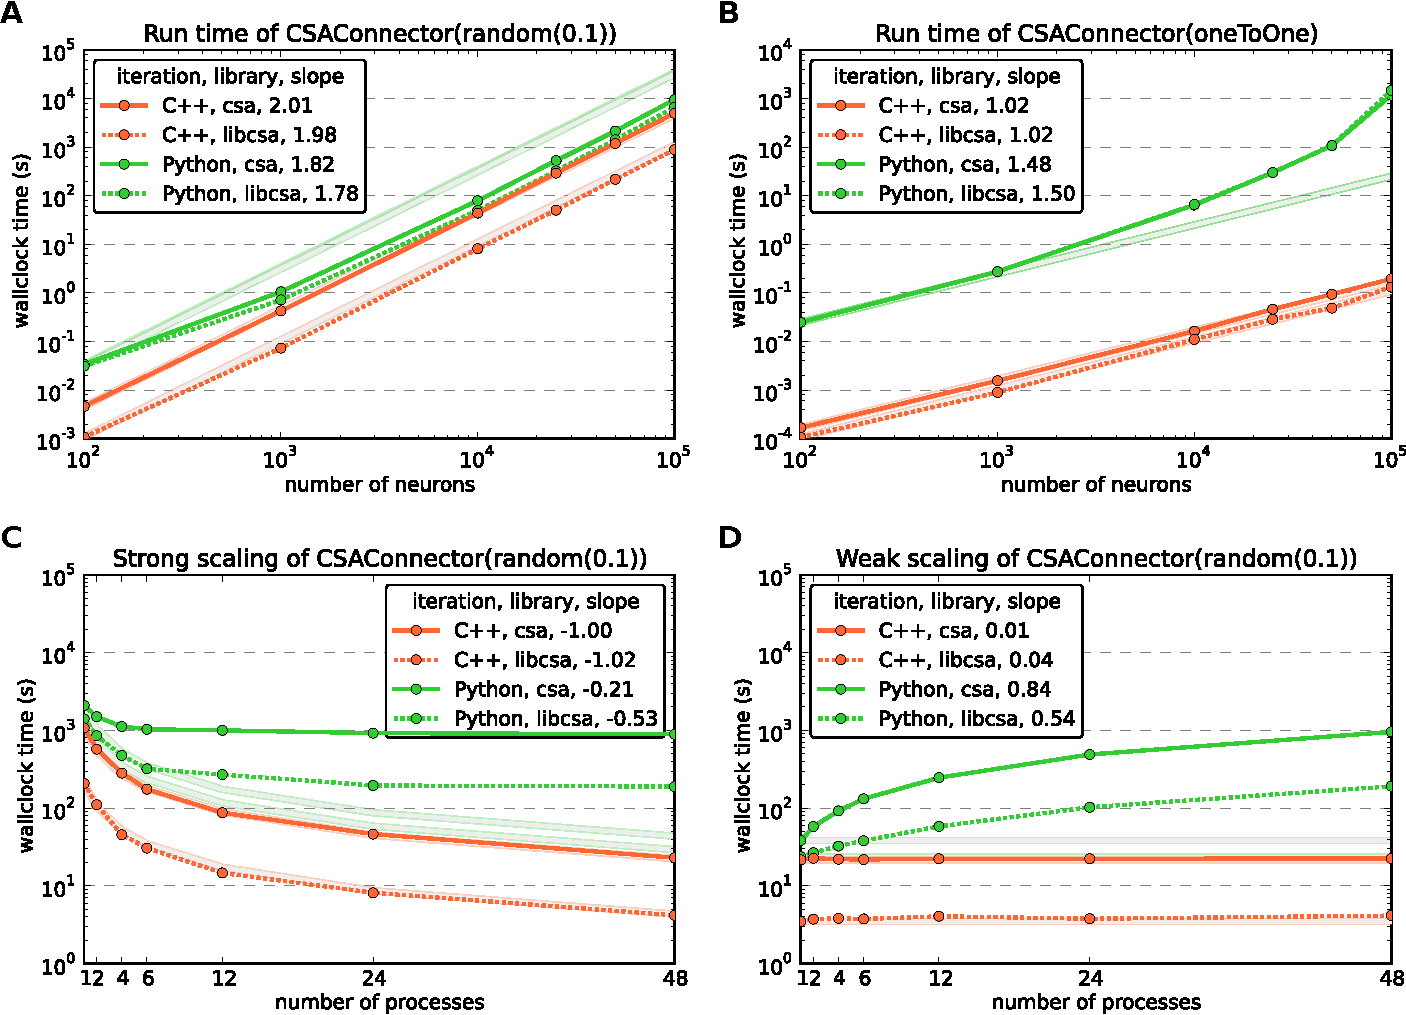
\includegraphics[scale=.7]{benchmarks/CSAConnector.pdf}
\caption{Benchmark results for the use of CSA in NEST through PyNN,
  comparing the two \texttt{CSAConnector} implementations explained in
  Section~\ref{sec:conn_gen_pynn} and two of the CSA implementations
  mentioned in Section~\ref{sec:csa}. Color and dash codes are given
  in the legends. Slope is the ratio of logarithms of the last and
  first data point shown. Pale lines denote the expected
  scaling. \textbf{A} shows the run time for connecting a network
  using CSAs \emph{random} mask with a probability of 0.1 for
  different numbers of neurons. This connector creates $O(n^2)$
  connections for $n$ neurons. The expected slope is thus
  2. \textbf{B} shows the same as in A, but using CSAs \emph{oneToOne}
  mask, which creates $O(n)$ connections for $n$ neurons and has an
  expected slope of 1. \textbf{C} shows a strong scaling experiment,
  wiring a network of 48,000 neurons using CSAs \emph{random} mask
  with a probability of 0.1 and varying the number of MPI processes
  from 1 to 48. The expected slope is -1, meaning that the run time
  drops linearly with the number of processes. \textbf{D} shows the
  results of a weak scaling experiment, increasing the number of
  connections by approx. $4.8 \cdot 10^6$ per additional MPI process
  for 1 to 48 processes. The expected slope is 0, as the load
  increases linearly with the number of
  processes.}\label{fig:pynn_benchmarks}
\end{figure}
\fi

The population size benchmarks (\Figure{4}{fig:pynn_benchmarks}A and
B) used one MPI process and varied the number of neurons from $10^2$
to $10^5$ with about one sample per order of magnitude. All tested
implementations of CSA (\verb|csa|, \verb|libcsa|) scale excellently
with slopes around 2 for the \emph{random} mask, independent of the
software layer (C++ or Python), on which the iteration was carried
out. However, in \Figure{4}{fig:pynn_benchmarks}, the vertical offsets
and the increasing slopes of the curves for the generic
\verb|CSAConnector| which iterates at the Python/PyNN level suggest
that the current implementation of this connector together with calls
through different software layers to setup individual connections adds
a significant overhead to the process of connection generation.

To demonstrate the scalability of the implementations, we carried out
both strong and weak scaling benchmarks, using CSA's \emph{random}
mask $\bar{\rho}(p)$ with a probability $p = 0.1$
(\Figure{4}{fig:pynn_benchmarks}C and D). For each of these, the
number of MPI processes was varied from 1 to 48.

In the strong scaling benchmark (\Figure{4}{fig:pynn_benchmarks}C),
the number of MPI processes was varied while keeping the total number
of neurons in the network fixed at $48000$. This resulted in
approx. 230 million connections being created. It is easily visible
that iteration of the CSA object at the Python level in the current
PyNN implementation of the original \verb|CSAConnector| is detrimental
to the scalability. In contrast, it is possible to obtain near perfect
scaling if the iteration of the CSA object is carried out from the C++
layer. Using the C++ implementation of CSA, it is, however, possible
to gain another order of magnitude compared to the Python version.

During the weak scaling benchmark (\Figure{4}{fig:pynn_benchmarks}C),
the number of MPI processes was varied while the work load was
increased by a fixed number of connections per additional process.
The number of connections grows quadratically with the number of
neurons when using CSA's \emph{random} mask with a fixed
probality. The number of neurons per process was thus increased with
the square root of the desired number of connections. In the realm of
natural numbers, this leads to a slight error, which was, however,
acceptable, with values between $-1.42$\permil and $+1.08$\permil.

\subsection{Comparison to native interfaces}

To compare the performance of the connection generator interface to
more traditional ways of setting up connectivity, we also performed
performance and scaling benchmarks of the native interfaces for random
connectivity in PyNN and NEST. \Figure{5}{fig:native_benchmarks}
contrasts CSA's \emph{random} mask with a probability of $0.1$ with
PyNN's \verb|FixedProbabilityConnector| (FPC) and NEST's function
\verb|RandomConvergentConnect| (RCC).

Note that NEST does not provide a Bernoulli trial based connection
scheme such as used by FPC in PyNN and the \emph{random} mask in CSA
(see Section~\ref{sec:structure}) and RCC was chosen because it is the
function that most closely resembles such a method. The use of RCC results,
however, in a bias towards the other methods over NEST, as it requires
iterative calls to RCC from the Python level, which entail a certain
overhead in SLI, PyNEST and the C++ implementation of RCC itself (data
not shown).

\ifdefined\INLINEFIGS
\begin{figure}[ht]
\centering
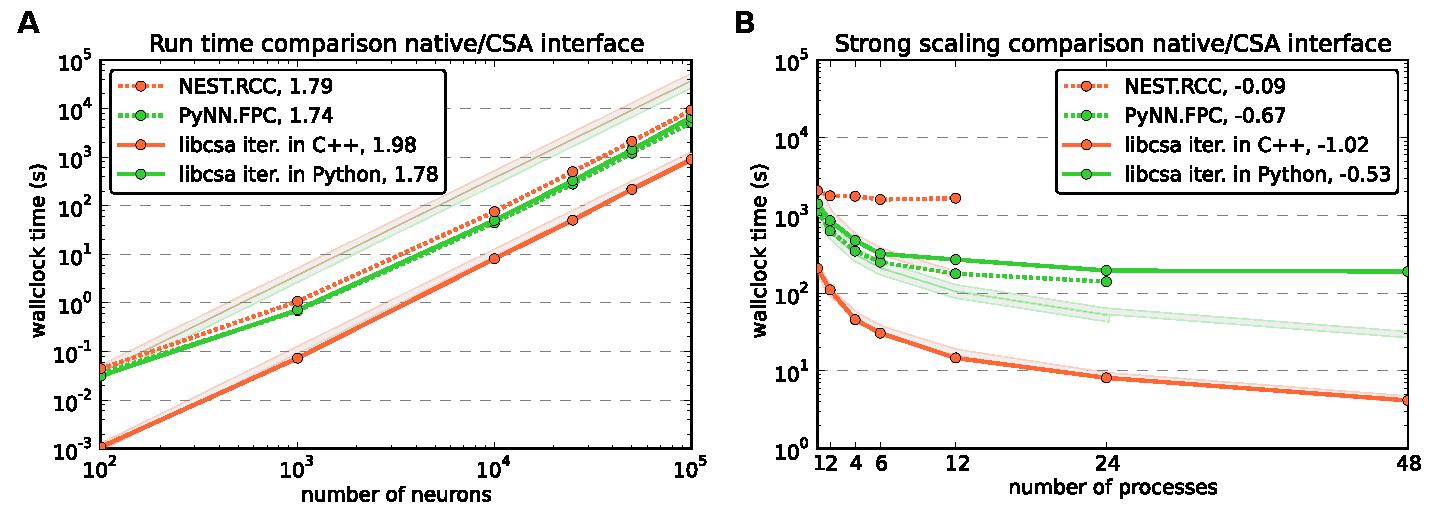
\includegraphics[scale=.7]{benchmarks/native_routines.pdf}
\caption{Benchmark results comparing the use of CSA in NEST through
  PyNN and the native interfaces for random connectivity in PyNN and
  NEST. Color and dash codes are given in the legends. Slope is the
  ratio of logarithms of the last and first data point shown. Pale
  lines denote the expected scaling. \emph{PyNN.FCC} corresponds to
  PyNN's \texttt{FixedProbabilityConnector}, \emph{nest.RCC} to NEST's
  function \texttt{RandomConvergentConnect}. \textbf{A} shows the run
  time for connecting a network of different numbers of neurons. The
  number of connections scales with $O(n^2)$ for $n$ neurons. The
  expected slope is thus 2. The data for libcsa is the same as shown
  in \Figure{4}{fig:pynn_benchmarks}A. \textbf{B} shows a strong
  scaling experiment, wiring a network of 48,000 neurons using CSAs
  \emph{random} mask with a probability of 0.1 and the corresponding
  native functions of PyNN and NEST. The experiment varies the number
  of MPI processes from 1 to 48. The expected slope is -1, meaning
  that the run time drops linearly with the number of processes. The
  data for libcsa is the same as shown in
  \Figure{4}{fig:pynn_benchmarks}C.}\label{fig:native_benchmarks}
\end{figure}
\fi

The population size benchmark (\Figure{5}{fig:native_benchmarks}A)
again used one MPI process and varied the number of neurons from
$10^2$ to $10^5$ with about one sample per order of magnitude. It
shows that all tested variants for setting up the connectivity scale
equally well with slopes slightly below 2. The offset between NEST's
RCC (written in C++, but called repeatedly from Python) to the CSA
object iterated in C++ can be attributed to overhead in the additional
software layers.

As in \Figure{4}{fig:pynn_benchmarks}C, the comparative strong scaling
benchmark shown in \Figure{5}{fig:native_benchmarks}B varied the
number of MPI processes while keeping the total number of neurons in
the network fixed at $48000$, resulting in a total of approx. 230
million connections being created. The results are consistent with the
data from \Figure{4}{fig:pynn_benchmarks}C in that scalability is
destroyed if additional interpreted software layers are involved and
that an iteration in C++ is favorable. The effect is even stronger for
RCC, because its use to create a number of connections corresponding
to that yielded by a Bernoulli trial scheme entails even more
iterations through the additional software layers.

\subsection{Benchmark environment}

The machine used for benchmarking was equipped with 4 12-core AMD
Operon 6174 (Magny Cours) processors, organized into 8 NUMA domains
with 6 cores each. Other than the choice of the number of MPI
processes in a NUMA-friendly way, no measures (like pinning of
processes to cores, altering the affinity of threads to cores, etc.)
were taken to avoid distortions of the results. Users are, however,
free to benefit from such techniques to improve the performance of
their simulations.

\subsection{Software versions and benchmark scripts}

All benchmarks were using \verb|csa| revision 119 from
\url{http://svn.incf.org/svn/csa}, \verb|libcsa| from an internal git
repository (\url{git@wand.pdc.kth.se:libcsa.git}, version 3ef2db519a),
the development version of PyNN from
\url{https://github.com/NeuralEnsemble/PyNN/} (version db76c748cd) and
NEST revision r10722 from the internal Subversion repository. The
\LaTeX{}  sources of this article, the benchmark scripts and all data we
obtained are available from
\url{https://github.com/mdjurfeldt/pns2csa}.

%----------------------------------------------------------------------

\section{Discussion and outlook}

We have developed and demonstrated a novel way to connect a simulator
and external connectivity-generating software through the connection
generator interface. It supports dynamic loading of connection
generators without the need for recompilation of either simulator or
generators. Benchmarks show good scaling when using Connection-set
Algebra libraries from NEST and PyNN. The availability of this and
associated interfaces lets users flexibly choose a
connectivity-generating library independently of the simulator used,
and thereby grants greater freedom for describing models.

The first version of the interface presented here was intentionally
made simple, as a proof of concept, and there are several possible
directions of development for its functionality. Currently, parameters
are passed as \verb|double|s. This could be generalized to other data
types.  For parallel simulators, connection generators may need access
to the MPI communicator.  Instead of using a fixed iteration order,
the order could be specified by the simulator. Iteration order could
also be unspecified, giving opportunities for more optimal iteration
on the part of the connectivity-generating library.  In order to
maintain backward compatibility as new revisions of the interface are
developed, interface versioning could be introduced.

One temporary limitation in the current implementations of the NEST
\verb|ConnectionGeneratorModule| and the PyNN \verb|CSAConnector| is
that value sets for the connection generator can only be used if its
arity is 0 or 2. This means that only values for weight and delay can
be generated by the connectivity-generating library. For many synapse
models, such as those with activity-dependent weights, it would be
beneficial to also set other parameters based on rules in the
connection generator.

At the moment, \verb|libneurosim| only contains the connection
generator interface and some auxilliary code. For the future, we are
planning to turn this into a community based effort to share common
interfaces and make it a generally useful library also for the
developers of other simulators than PyNN and NEST.

The differences in run time and scalability between an iteration of
the connection description in Python on the one hand and the CSA
object iterated on the C++ level on the other suggests that a compact
description of connectivity iterated solely at the level of the
simulator indeed has a huge impact. NEST and other simulators can thus
greatly benefit from the availability of compact descriptions such as
enabled by the connection generator interface.

%----------------------------------------------------------------------

\section*{Conflict-of-Interest Statement}
The authors declare that the research was conducted in the absence of
any commercial or financial relationships that could be construed as a
potential conflict of interest.

\section*{Acknowledgement}
This work was partially done under the INCF Multiscale Modeling
Program. It is partially supported by the Helmholtz Association: HASB
and portfolio theme SMHB, the Jülich Aachen Research Alliance (JARA),
the VSR computation time grant JINB33 on the JUQUEEN supercomputer in
Jülich, and EU Grant 269921 (BrainScaleS). The authors would like to
thank Randall Munroe of \url{http://www.xkcd.org} for granting the
permission to use one of his drawings in
Figure~\ref{fig:sequence_diagram_nest}.

\bibliographystyle{frontiersinSCNS&ENG}
\bibliography{pns2csa13}

\end{document}
